\documentclass[border=10pt]{standalone}

\usepackage{tikz}
\usepackage{tikzsymbols}
\usetikzlibrary{calc,patterns,shapes.geometric}

\def\centerarc[#1](#2)(#3:#4:#5){\draw[#1] ($(#2)+({#5*cos(#3)},{#5*sin(#3)})$) arc (#3:#4:#5);}

\begin{document}
	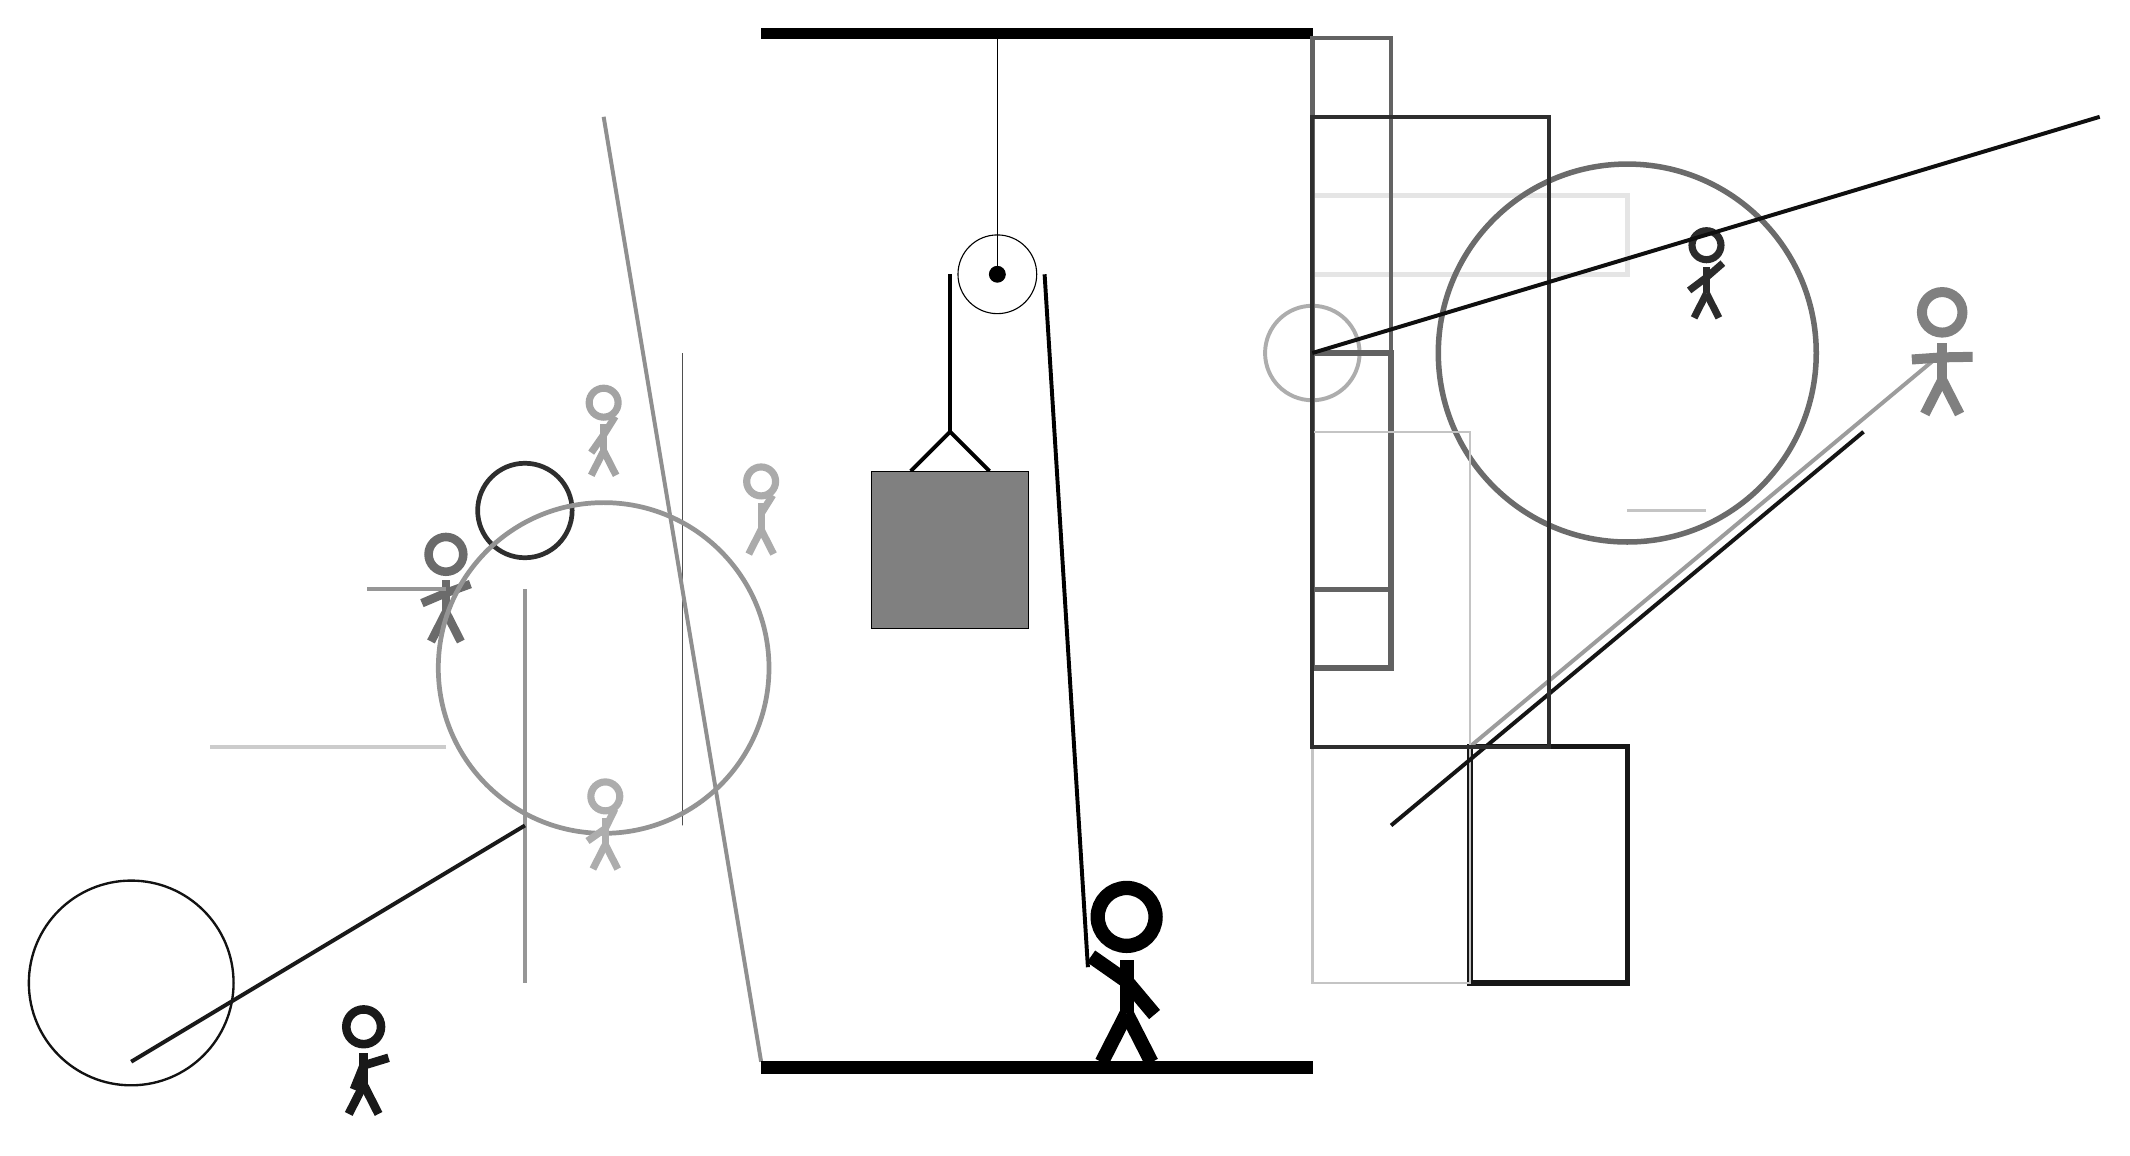
\begin{tikzpicture}
		%%%%% START %%%%%
		
		\draw[fill=black] (-2, 10) rectangle (5, 10.125);
		
		\draw (1, 7) circle (0.5);
		\draw[fill=black] (1, 7) circle (0.1);
		\draw (1, 10) -- (1, 7);
		
		\draw[line width=0.5mm] (-0.1, 4.5) -- (0.4, 5.0) -- (0.9, 4.5);
		\draw[fill=black!50] (-0.6, 4.5) rectangle (1.4, 2.5);
		
		\draw[line width=0.5mm] (0.4, 7) -- (0.4, 5.0);
		\centerarc[line width=0.5mm](1, 7)(0:180:0.6);
		\draw[line width=0.5mm](1.6, 7) -- (2.15, -1.8);
		
		\node[line width=0.2mm, color=black!58] at (-6, 3) {\Strichmaxerl[6][23][20]};
		
		\draw[line width=0.7mm, color=black!91] (7, 1) rectangle (9, -2);
		\draw [line width=0.5mm, color=black!32](5, 6) circle (0.6);
		\node[line width=0.2mm, color=black!36] at (-4, 5) {\Strichmaxerl[5][55][58]};
		\draw[line width=0.2mm, color=black!69] (-3, 6) rectangle (-3, 0);
		\node[line width=0.2mm, color=black!83] at (10, 7) {\Strichmaxerl[5][37][41]};
		\draw[line width=0.5mm, color=black!39](7, 1) -- (13, 6);
		\draw [line width=0.6mm, color=black!82](-5, 4) circle (0.6);
		\draw[line width=0.7mm, color=black!10] (5, 7) rectangle (9, 8);
		
		\draw[line width=0.5mm, color=black!20](-6, 1) -- (-9, 1);
		
		\draw[line width=0.6mm, color=black!61] (5, 10) rectangle (6, 3);
		\node[line width=0.4mm, color=black!90] at (-7, -3) {\Strichmaxerl[6][68][17]};
		\draw[line width=0.5mm, color=black!41](-7, 3) -- (-6, 3);
		
		\draw [line width=0.7mm, color=black!58](9, 6) circle (2.4);
		\draw[line width=0.5mm, color=black!44](-2, -3) -- (-4, 9);
		\draw[line width=0.7mm, color=black!62] (6, 2) rectangle (5, 6);
		\draw [line width=0.3mm, color=black!93](-10, -2) circle (1.3);
		\draw[line width=0.3mm, color=black!23] (5, 5) rectangle (7, -2);
		\draw[line width=0.5mm, color=black!92](6, 0) -- (12, 5);
		\draw[line width=0.5mm, color=black!41](-5, 3) -- (-5, -2);
		\node[line width=0.4mm, color=black!33] at (-2, 4) {\Strichmaxerl[5][90][58]};
		\draw[line width=0.5mm, color=black!23](10, 4) -- (9, 4);
		\draw [line width=0.6mm, color=black!42](-4, 2) circle (2.1);
		\draw[line width=0.5mm, color=black!82] (5, 9) rectangle (8, 1);
		\draw [line width=0.2mm, color=black!47](8, 2) circle (0.0);
		\draw[line width=0.5mm, color=black!90](-5, 0) -- (-10, -3);
		\draw[line width=0.5mm, color=black!94](5, 6) -- (15, 9);
		\node[line width=0.2mm, color=black!32] at (-4, 0) {\Strichmaxerl[5][35][64]};
		
		\node[line width=0.6mm, color=black!50] at (13, 6) {\Strichmaxerl[7][4][1]};
		
		\node at (2.6, -1.9) {\Strichmaxerl[10][-35][-50]};
		
		\draw[fill=black] (-2, -3) rectangle (5, -3.15);
		
		%%%%% END %%%%%
	\end{tikzpicture}
\end{document}